\documentclass[14pt,a4paper]{extarticle}

\usepackage[utf8]{inputenc}
\usepackage[T1]{fontenc}
\usepackage[english]{babel}
\usepackage{mathptmx}

\usepackage[
    top=2cm,
    bottom=2cm,
    left=3cm,
    right=1.5cm
]{geometry}

\usepackage{setspace}
\usepackage{indentfirst}
\usepackage{enumitem}
\usepackage{booktabs}
\usepackage{longtable}
\usepackage{array}
\usepackage{hyperref}
\usepackage{xcolor}
\usepackage{titlesec}
\usepackage{caption}
\usepackage{tabularx}
\usepackage{amsmath}
\usepackage{amssymb}
\usepackage{float}
\usepackage{makecell}
\usepackage{graphicx}
\graphicspath{{figures/}}
\usepackage{csquotes}
\usepackage{microtype}
\usepackage[
    backend=biber,
    style=apa,
    natbib=true
]{biblatex}
\addbibresource{Bib additions.bib}

% Square-bracket APA citations: [Author, Year].
% All existing \cite{...} commands in the text remain unchanged.
\DeclareDelimAlias[squarecite]{finalnamedelim}[parencite]{finalnamedelim}
\DeclareCiteCommand{\squarecite}[\mkbibbrackets]
  {\usebibmacro{cite:init}%
   \usebibmacro{prenote}%
   \toggletrue{apa:inpcite}}
  {\usebibmacro{citeindex}%
   \usebibmacro{cite}%
   \usebibmacro{cite:post}}
  {}
  {\usebibmacro{postnote}%
   \togglefalse{apa:inpcite}}
\DeclareMultiCiteCommand{\squarecites}[\mkbibbrackets]{\squarecite}
  {\setunit{\multicitedelim}}
\let\cite\squarecite
% Apply the required bracket format to narrative citation commands as well.
\let\textcite\squarecite

\newcommand{\safeincludegraphics}[2][]{%
  \IfFileExists{#2}{%
    \includegraphics[#1]{#2}%
  }{%
    \IfFileExists{figures/#2}{%
      \includegraphics[#1]{figures/#2}%
    }{%
      \fbox{\parbox{0.86\linewidth}{\centering Missing figure file: \texttt{\detokenize{#2}}}}%
    }%
  }%
}

\newcolumntype{L}[1]{>{\raggedright\arraybackslash}p{#1}}

\hypersetup{
    colorlinks=true,
    linkcolor=black,
    urlcolor=blue,
    citecolor=black
}

\onehalfspacing
\setlength{\parindent}{1.25cm}
\setlength{\parskip}{0pt}
% Absorb residual right-margin overflow in justified prose (long identifiers,
% inline math) without altering wording.
\setlength{\emergencystretch}{3em}

\setlist[itemize]{leftmargin=1.5em}
\setlist[enumerate]{leftmargin=1.8em}

\titleformat{\section}{\large\bfseries}{\thesection.}{0.5em}{}
\titleformat{\subsection}{\normalsize\bfseries}{\thesubsection.}{0.5em}{}
\titleformat{\subsubsection}{\normalsize\itshape}{\thesubsubsection.}{0.5em}{}
\newcommand{\code}[1]{\texttt{\detokenize{#1}}}
% Make snake_case identifiers wrap when a line would otherwise overflow (purely a
% line-breaking aid: a reluctant break after each underscore, no glyph change; no
% section title or caption uses \_, so PDF bookmarks are unaffected).
\newcommand{\snakebreak}{\renewcommand{\_}{\textunderscore\allowbreak}}
\begin{document}
\snakebreak

% Anonymous title page: no author, affiliation, or city.
\hypersetup{pageanchor=false}
\begin{titlepage}
\begin{center}
\vspace*{3.0cm}
{\Large\bfseries Social Desirability in Large Language Model Responses:
A Vignette-Experimental Study of Synthetic Respondents\par}
\vspace{2.4cm}
{\normalsize Field of Research: Sociology\par}
\vspace{1.2cm}
{\normalsize Keywords: large language models; synthetic respondents;
social desirability; vignette experiments; system prompts\par}
\vfill
{\normalsize 2026\par}
\end{center}
\end{titlepage}
\hypersetup{pageanchor=true}

\tableofcontents
\clearpage

\begin{abstract}
We examine how system prompts affect large language models as synthetic respondents in four vignette experiments: coercive interrogation, charitable giving, energy conservation, and bribery. We compare responses with published human treatment effects and analyze final answers, verbalized reasoning, and exploratory hidden states. Replication of human effects is inconsistent across tasks and models. Anti-sanitization prompts sometimes produce large response shifts, whereas positive and negative research-consequence framing yields smaller, less consistent changes. Reasoning annotations shift with prompts and correlate with answers, but do not identify causal mechanisms. Moving responses away from socially approved positions does not reliably improve correspondence with human experimental effects.

The authors used AI to assist with code development, data analysis workflows, data markup and to improve the language and translation of the text. The authors reviewed and edited the output and take full responsibility for the content.
\end{abstract}

\section{Introduction}

Large language models (LLMs) are used to simulate survey respondents and pilot experimental designs \cite{argyle2023,horton2023,dillion2023}. Plausible answers, however, do not establish replication of human treatment effects. Socially sensitive vignettes sharpen this problem: human responses may reflect social desirability, while LLM outputs also depend on safety alignment and instructions \cite{tourangeau2007,krumpal2013,salecha2024,sharma2023}. Moving an answer away from a socially approved position does not necessarily make it more human-like.

We study four adapted experiments: Hassner's coercive interrogation, Savary and Goldsmith's charitable giving, Bolsen et al.'s energy conservation, and Corbacho et al.'s corruption information. We compare synthetic treatment contrasts with published human benchmarks and estimate the effects of additional system prompts. Prompts are treated as experimental inputs, not validated corrections for social desirability bias.

\textbf{Research question.} How do system-prompt stimuli affect LLM answers, verbalized reasoning, and internal representations in socially sensitive vignette experiments?

\textbf{Goal and objectives.} We (i) compare original treatment contrasts with human benchmarks; (ii) estimate stimulus shifts and treatment-by-stimulus differences; (iii) analyze annotated arguments and their associations with answers; and (iv) explore stimulus and answer information in a separate local model's hidden states. These levels are distinct: textual associations and representational decodability do not establish causal mechanisms.

Behavioral responses and verbalized reasoning are analyzed across all four cases; hidden-state analysis concerns only the two initial cases and a separate local model.


\section{Literature Review}

\subsection{LLMs as synthetic respondents}

LLMs offer inexpensive ways to pilot surveys and experimental vignettes. Early work explored demographic conditioning and \emph{algorithmic fidelity} \cite{argyle2023}, classical experimental replication \cite{aher2023}, and simulated economic agents \cite{horton2023}. Their value depends on replicating human treatment contrasts. Replication studies find some directional agreement alongside exaggerated magnitudes, compressed variation, and weaker correspondence in socially sensitive domains \cite{cui2025,bisbee2024,santurkar2023,rottger2024}. We benchmark synthetic treatment contrasts against human studies.

\subsection{Social desirability and instruction sensitivity}

Social desirability bias (SDB) is response distortion associated with perceived acceptability. Survey theory distinguishes impression management from self-deceptive enhancement and emphasizes question sensitivity, privacy, and administration mode \cite{crowne1960,paulhus1984,tourangeau2007,krumpal2013}. Indirect elicitation and anonymity can reduce some human response pressures \cite{nederhof1985,horiuchi2022}; system prompts are not established equivalents of these survey methods.

LLM behavior introduces additional explanations. Models may favor socially approved answers, conform to perceived user expectations, or respond to safety-related training and instructions \cite{salecha2024,sharma2023}. Survey prompts and response formats can also change their outputs \cite{tjuatja2024}. A shift away from a socially approved answer therefore need not represent reduced human-like SDB. We distinguish behavioral steering from human-effect replication.

\subsection{Consequence framing versus gain--loss framing}

Human studies establish that framing can affect decisions, but the magnitude varies substantially across problem designs \cite{kuhberger1998}. Reviews of persuasive messages likewise do not find a general advantage of loss over gain framing \cite{okeefeJensen2006}. Importantly, those studies manipulate how a choice or message is presented to human respondents. Our N$-$/N$+$ conditions instead frame consequences in \emph{system-level instructions} to a synthetic respondent, rather than presenting matched gains and losses within the vignette. Their effects need not replicate classic gain--loss framing.

\subsection{Reasoning and internal representations}

Chain-of-thought prompting can alter generated outputs \cite{wei2022,kojima2022}, but verbalized reasoning is not a validated record of a model's internal causal process. We distinguish final answers, coded argumentative content, and hidden-state measurements. Annotation can identify associations between expressed arguments and responses, conditional on its reliability. Hidden-state probes offer a separate representational diagnostic; in our design, they concern a different local model and cannot be treated as a direct explanation of API-model behavior.

\subsection*{Research contribution}

We compare human treatment benchmarks and prompt effects in four domains, including verbalized reasoning, and explore hidden states in the two initial cases. Differences across models and formats do not establish human validity.


\section{Research Design and Data}

\subsection{Case selection and experimental treatments}

We study four published \emph{attitude-expression} vignette experiments. Unlike autobiographical self-report questions, these tasks ask for judgments about externally described situations. This choice permits controlled variation of vignette treatments without assigning demographic identities or personal histories to the model. The original cases also differ in the normative direction of the response: endorsement of coercive interrogation is socially disapproved, whereas charitable giving is socially approved. We use this contrast to investigate whether system-prompt stimuli have similar or domain-specific effects.

\textbf{Hassner: coercive interrogation.} In the Hassner experiment \cite{hassner2023}, models evaluate the use of sleep deprivation in interrogating a terrorism suspect. The four conditions are a base case, modest expected intelligence value, protracted duration, and their combination. The response is binary (support versus opposition). Opposition is treated as the \emph{normatively approved response direction} for descriptive comparisons, not as a verified measure of an individual respondent's latent attitude.

\textbf{Savary and Goldsmith: charitable donation.} In the Savary and Goldsmith experiment \cite{savary2020}, models report willingness to donate \$5 on a five-point scale. The three vignette conditions are private donation, public recognition, and public recognition combined with an additional social benefit. Greater stated willingness is the normatively approved response direction. The public-recognition treatment is also substantively important because it may alter the interpretation of donation as altruism or reputational signaling.

\paragraph{Bolsen et al.: energy conservation.}
The third experiment adapts Bolsen et al.'s energy-conservation design \cite{bolsen2014}. Its nine treatment cells combine attribution of responsibility (government, individuals, or neither) with economic-cost, environmental-benefit, or no consequence framing. Models rate likelihood of investing in home insulation or weatherization on a seven-point scale. We examine original treatment-versus-control comparisons as well as attribution-by-consequence contrasts. The dependent variable measures stated willingness, not observed investment.

\paragraph{Corbacho et al.: bribery and institutional information.}
The fourth experiment adapts Corbacho et al. \cite{corbacho2016}, comparing a control with information about corruption prevalence and an institutional-inefficiency placebo. Respondents indicate whether they would offer a bribe to avoid a fine, selecting True, False, or Prefer not to respond. These are three nominal outcomes; refusal is not interchangeable with unwillingness. The source paper reports direct-response and privacy-adjusted comparisons with different estimands. Our prompt adaptation does not reproduce its original crosswise-response procedure.

Because original elicitation procedures and outcomes differ, we compare treatment directions without pooling numerical effect sizes. Matching a direction does not establish matching response distributions or mechanisms.

\subsection{Prompt structure and unit of observation}

Original treatments vary user-facing vignettes; stimuli modify survey-task system instructions. No demographic persona is assigned in the principal behavioral design. Stimulus wording is identified from available generation configurations; unverified historical H--M wording is not quoted.

Each run generates an answer and, where available, a linked reasoning trace. Repeated completions in the same model--experiment--treatment--stimulus cell measure within-cell variation, not independent human respondents; inference must respect that grouping.

\subsection{Models, decoding, and analytical samples}

The behavioral corpus uses four API models (short names GLM and Kimi refer to GLM-4.6 and Kimi-K2-Thinking): \texttt{moonshotai/kimi-k2-thinking}, \texttt{z-ai/glm-4.6}, \texttt{qwen/qwen3.5-9b}, and \texttt{minimax/minimax-m2.5}. These models were selected pragmatically for the availability of final answers and reasoning traces; they do not constitute a representative sample of all LLMs. Local \texttt{Qwen3-8B} hidden states are analyzed separately.

The principal generation regime uses temperature $T=0.01$, with a separate no-stimulus comparison at $T=1.0$. Low temperature may compress within-cell variation; temperature contrasts are not human benchmarks.

The historical corpus reports 15{,}680 raw runs, 12{,}434 retained rows, and 11{,}040 main $T=0.01$ observations. Historical totals follow the available reconciled master-table copy; the H--M family was collected only for GLM and Kimi.

\section{System-Prompt Stimuli}

\subsection{Conceptual role}

System-prompt stimuli modify the instructions surrounding a fixed vignette. They are intended to discourage normatively polished or sanitized answers, but their observed effects are described here as \emph{stimulus-induced response shifts}, not as established reductions in social desirability bias. The direction of a shift is evaluated relative to the \emph{normatively approved response direction} in each case. A shift away from that direction does not, on its own, establish greater correspondence with human responses.

The historically implemented stimulus set includes the no-stimulus baseline, two core conditions (A and C), and the extended H--M family. A emphasizes the costs of sanitized answers; C includes an explicit anti-overcorrection qualification. The H--M family varies the stated target of consequences or benefits (science versus a company; personal or institutional benefit versus public good) and the valence of the framing (negative consequences versus positive benefits). Labels describe intended functions, not mechanisms.

\subsection{Historical stimulus conditions and coverage}

\begin{table}[htbp]
\centering
\caption{Historical stimulus families and interpretation}
\label{tab:stimuli_editorial}
\begin{tabularx}{\textwidth}{L{2.5cm}X}
\toprule
\textbf{Condition} & \textbf{Interpretation and limitation}\\
\midrule
No stimulus & Baseline survey task without an additional experimental system-prompt stimulus.\\
A & Anti-sanitization instruction invoking consequences for research quality; paraphrase, not a verbatim prompt.\\
C & Core realism instruction with an anti-overcorrection qualification; not a neutral control matched to A on all dimensions.\\
H--K & Negative consequence framing with different stated recipients or beneficiaries; fielded in a subset of models.\\
L--M & Positive benefit framing with different stated recipients or beneficiaries; fielded in a subset of models.\\
\bottomrule
\end{tabularx}
\end{table}

The existing coverage matrix contains H--M records for \emph{both} Hassner and Savary. However, the available project reconstruction provides semantic descriptions rather than verified verbatim H--M prompt strings. We therefore avoid verbatim claims about H--M wording and do not treat this family as an orthogonal factorial design.

N0, N$-$, and N$+$ are also used in the new experiments and the Hassner/Savary extension; N0 is distinct from historical no stimulus.

\subsection{Exact N-series stimuli and reference conditions}
N0, N$-$ and N$+$ are stimulus labels, not sample sizes. N0 is the neutral-realism reference; N$-$ and N$+$ append negative or positive consequences for research accuracy. The following wording was used:

\begin{quote}\small
\textbf{N0:} Your task is to answer the survey question as a plausible human respondent might answer under the conditions described. Focus on the respondent's likely judgment rather than on recommending what anyone should do.

\textbf{N$-$ addition:} If your response does not realistically reflect how a human respondent might answer, the study may draw inaccurate conclusions about human behavior and become less useful for future research.

\textbf{N$+$ addition:} If your response realistically reflects how a human respondent might answer, the study may draw accurate conclusions about human behavior and become more useful for future research.
\end{quote}

The historical no-stimulus baseline, separately collected \texttt{none} baseline, and instruction-bearing N0 are distinct; they must not be pooled as equivalent controls. A/C and H--M are described by function above; exact historical H--M strings are not independently verified.

\subsection{Analytical contrasts}

The behavioral analysis distinguishes three comparisons: (i) original vignette-treatment contrasts within a fixed prompt condition; (ii) stimulus-induced shifts relative to a no-stimulus or explicitly specified reference condition; and (iii) changes in original treatment contrasts across stimulus conditions. Attribute-level comparisons are interpreted as conditional associations unless the compared prompts isolate the attribute of interest and have sufficient balanced coverage. Reasoning and hidden states remain complementary diagnostics.


% Editorial draft: replaces Reasoning-Trace Annotation and Analytical Strategy.
% Historical and new-case behavioral and reasoning analyses.
\section{Analytical Strategy}

Each generation belongs to a design cell; repeated low-temperature completions are not independent human respondents.

\subsection{Behavioral outcomes}

Hassner endorsement is binary (logit and penalized-logit sensitivity); Savary uses a five-point willingness score (OLS, ordinal, and threshold sensitivities); Bolsen uses a seven-point investment scale (cell means and ordinal distributions). Corbacho has three nominal outcomes---True, False, and refusal---which are never collapsed into an ordered score. We estimate original vignette-treatment contrasts within stimulus and model, stimulus shifts within original treatments, and their interactions. The principal reference is historical no stimulus, fresh \texttt{none}, or new neutral realism N0, as appropriate; these are distinct conditions.

Pairwise Holm corrections and broader Benjamini--Hochberg adjustments address multiplicity. Historical models use heteroskedasticity-robust and design-cell-clustered checks. Low-temperature repetitions, quasi-separation and saturated cells constrain conventional uncertainty estimates. The new-experiment analysis uses model-specific cell contrasts, ordinal/nominal distribution checks and conditional block resampling; the latter does not yield uncertainty for a human population. Historical H--M prompt-attribute regressions are exploratory because the observed prompt packages do not isolate framing valence or beneficiary in a full factorial. Fresh \texttt{none} versus N-series comparisons may also reflect differences in run timing and provider routing.

\subsection{Verbalized reasoning}

LLM-based annotation (\texttt{gpt-5.4-mini}) retained 8,638 historical records; its categories encode three-level argument centrality, signed direction where defined, and style. A 27-trace expert-coded subset shows uneven agreement. The Bolsen/Corbacho batch contains 1,398 eligible traces over selected original treatments, and instead encodes binary category presence with signed direction where applicable. These schemes are not pooled as if they measured identical centrality. We estimate stimulus-related changes in category prevalence and, separately, argument direction among occurrences; undefined direction is not assigned zero. Within-cell regressions relate category presence to final outcomes with model, treatment, stimulus and version controls. Associations between co-generated traces and responses are not causal mediation. For rare and near-constant categories, estimates can be unidentified or imprecise.

\subsection{Local hidden-state exploration}

A separate Qwen3-8B study records 37 hidden-state outputs (embeddings plus 36 layers), each 4,096-dimensional, for last tokens for 98 runs under a different prompt inventory. Layer-wise distances, centered kernel alignment, matched trajectory contrasts, and predictive probes are descriptive diagnostics, not direct evidence of a mechanism in the API models. Observable shifts do not imply human validity.

\section{Results}

\subsection{Final answers: heterogeneous models and systematic prompt shifts}

Responses differ substantially by API model. Across the reported $T=0.01$ analytical sample, Hassner endorsement rates range from 10.3\% (Minimax) to 67.5\% (GLM-4.6), while Savary mean willingness ranges from 3.33 (Kimi) to 3.73 (Qwen). The Hassner treatment-by-model specification also improves model fit (McFadden pseudo-$R^2$: $0.507$ to $0.543$; $\Delta\mathrm{AIC}=-304$). Model identity therefore matters for both response levels and sensitivity to vignette manipulations. These rates are not balanced model comparisons.

In the no-stimulus Hassner condition, support for sleep deprivation decreases from 44.6\% in the control to 19.3\% with protracted duration, 12.2\% with modest intelligence value, and 1.0\% with both modifications. These directions agree with the human experimental benchmark. In Savary, by contrast, the LLM mean rises from 3.39 in the private condition to 3.73 with public recognition and 4.09 with added social benefit. The increment associated with social benefit is directionally consistent with the source experiment, but the private-to-public increase reverses the human finding: public recognition \emph{reduced} willingness in the original study. Replication is therefore domain-dependent.

All eight historical system-prompt stimuli are associated with shifts \emph{away from the normatively approved response direction} in the pooled descriptive comparisons. In Hassner, the no-stimulus endorsement rate is 19.1\%; it is 41.6\% under C, 72.1\% under A, and ranges from 56.4\% to 90.0\% across H--M. In Savary, mean willingness is 3.74 without a stimulus, 3.44 under C, 3.32 under A, and 3.14--3.35 across H--M (Table~\ref{tab:incentive-means}). These are \emph{socially desirable response patterns} and \emph{stimulus-induced response shifts}, not direct estimates of human-style SDB or its mitigation.

The comparisons require a coverage qualification: H--M were fielded only on Kimi and GLM-4.6, while the baseline and core conditions have broader model coverage. Thus the displayed pooled means are useful descriptive summaries, but differences involving H--M are not automatically like-for-like causal estimates. In the historical attribute regression restricted to the two-model subsample, positive-framed L/M prompts are associated with substantially higher Hassner endorsement than negative-framed H--K (reported OR $\approx15$, $p<0.001$) and a smaller decrease in Savary willingness (reported $\beta=-0.13$, $p=0.02$). Because the observed prompts do not form a complete matched factorial, these are associations between prompt packages, not isolated effects of framing valence. Nonsignificant recipient and beneficiary coefficients do not establish that those attributes are inert.

Treatment-by-stimulus contrasts also vary: the original analysis reports moderation in some conditions, without reversal of the sign of the original Hassner treatment contrasts. In Savary, the private-to-public contrast remains positive across the eight historical stimuli (reported range $+0.05$ to $+0.26$), so none reproduces the human reversal under the tested settings. This result identifies a limitation of the \emph{observed prompts}, not a general impossibility of eliciting self-signaling-related reasoning.

\paragraph{Historical-data consistency.}
Reprocessing the historical master table yields 11,040 observations in 168 cells. Sixteen cell estimates differ from a prior export, without reversing treatment directions. The historical input snapshot and some temperature metadata could not be fully matched across exports.

\subsection{Separate no-incentive baseline: Hassner and Savary}

A separate low-temperature October 2026 run without an additional incentive section produced 698 valid answers from 700 requests. In Hassner, GLM control endorsement is 1.000, falling to 0.673 (duration), 0.360 (modest intelligence), and 0.040 (both); Kimi's corresponding rates are 0.571, 0.140, 0, and 0. In Savary, private/public/social-benefit means are 3.48/3.92/4.42 (GLM) and 3.34/3.66/4.00 (Kimi). Both models preserve the historical treatment-effect directions, including Savary's public-recognition reversal relative to humans. The new \texttt{none} sample is not pooled with historical runs; its contrasts against later N-series runs are descriptive because inference-provider routing and execution time differed.

\subsection{N-series behavioral extension: Hassner and Savary}

The N0/N$-$/N$+$ extension yields 2,065 valid answers from 2,100 requests (Kimi 1,043; GLM 1,022). In Savary, N0 relative to the separate \texttt{none} run lowers mean willingness by 0.15 points for Kimi (95\% CI $[-0.23,-0.06]$, Holm $p=0.013$) and by 0.12 for GLM (Holm $p=0.339$). Compared with N0, both additional framings raise Kimi's mean by about 0.09, but lower GLM's by 0.14 (N$-$) and 0.21 (N$+$). The GLM N$+$ shift is $-0.213$ ($[-0.320,-0.107]$, Holm $p=0.00117$); the corresponding GLM--Kimi difference in shifts is $-0.307$ ($[-0.447,-0.167]$).

In Hassner, mean N$+$--N0 changes are $-6$ percentage points (pp) for Kimi (95\% CI $[-11.65,0.18]$; Holm $p=0.335$) and $+4$ pp for GLM (Holm $p=1$). However, Kimi's control endorsement falls from 72\% under N0 to 46\% under N$+$, an exploratory $-26$ pp local shift that changes treatment contrasts. Twenty-seven transport failures left only 23 of 50 valid GLM duration responses under N$-$. The Kimi mean contrast attenuates to about $-2$ pp after provider adjustment. Thus near-symmetric framings do not yield a universal effect, and cross-run contrasts cannot be assigned solely to prompt wording.

\subsection{Additional experiments: Bolsen and Corbacho}

\paragraph{Sample and comparability.}
The two new experiments contain 6,034 saved generations, 6,000 of which satisfy parsing and scale checks. GLM-4.6 and Kimi-K2-Thinking cover the full treatment-by-stimulus design; Qwen3.5-9B contributes only 33 valid Bolsen control/A responses and is excluded from the principal comparisons. The realized prompt conditions are A, C, N0, N$-$, and N$+$. N0 is a neutral realism instruction, not the historical no-incentive baseline; these references must not be equated.

\paragraph{Bolsen: partial directional replication and model heterogeneity.}
Under N0, both models' control means are 5.000 on the seven-point investment scale. Government attribution lowers investment likelihood by 0.840 points for GLM and 1.800 for Kimi, compared with approximately $-0.370$ in the published human contrast. Cost framing lowers it by 1.060 and 0.600 points, compared with a published contrast of approximately $-0.360$. The combined individual-attribution and environmental-benefit condition is only 0.020 points above control for either model, versus approximately $+0.450$ in the human study. Agreement in sign thus coexists with sizeable discrepancies in magnitude (Table~\ref{tab:bolsen-new-contrasts}). Published human contrasts are reconstructed from rounded means, and exact comparability is limited.

The factorial pattern is also heterogeneous. At N0, the individual-by-environment interaction is 0.000 for GLM and $-0.180$ for Kimi, against approximately $+0.120$ in the reported human means. Averaging equally across the nine treatments, A changes GLM's mean by $+0.168$ relative to N0 but Kimi's by $-0.665$; the corresponding C shifts are $+0.257$ and $-0.097$. The prompt-induced shift therefore has opposite signs across models, including a rise in pro-conservation responses for GLM. In Kimi, the cost-minus-control contrast changes from $-0.600$ under N0 to $+0.080$ under A. These shifts neither guarantee greater human correspondence nor support a uniform de-sanitization claim.

% BEGIN APPROVED FIGURE INSERTION: balanced levels
\noindent Figure~\ref{fig:balanced-stimulus-levels}.
\begin{figure}[H]
\centering
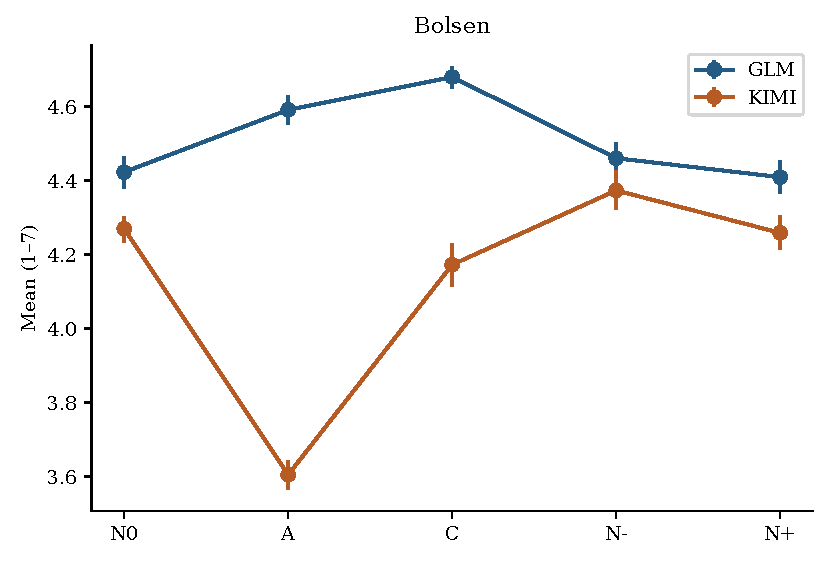
\includegraphics[width=0.92\linewidth]{figures/05_bolsen_panel.pdf}\\[0.3em]
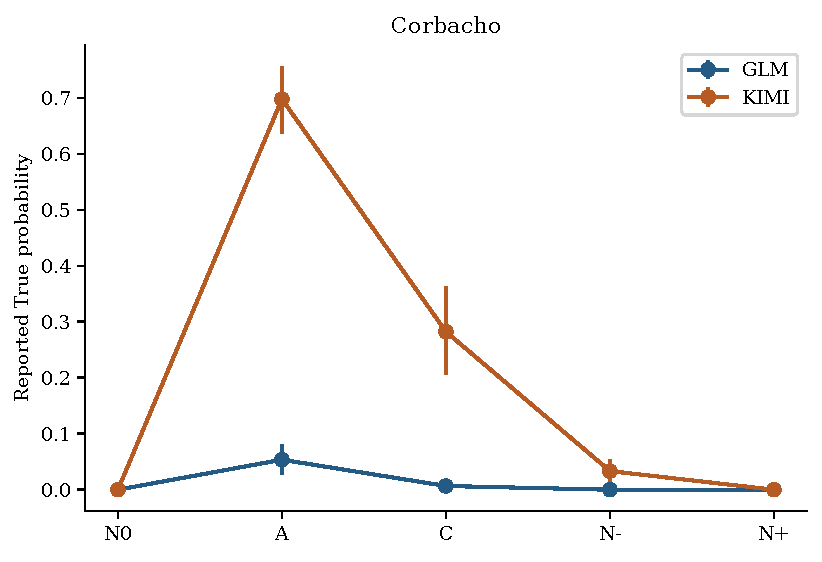
\includegraphics[width=0.92\linewidth]{figures/05_corbacho_panel.pdf}
\captionsetup{font=small}
\caption{Treatment-balanced response levels by model and prompt. Equal treatment weights; pointwise block-10 conditional reference intervals. N0 is neutral realism. Bolsen: mean on the 1--7 scale; Corbacho: True probability.}
\label{fig:balanced-stimulus-levels}
\end{figure}
% END APPROVED FIGURE INSERTION

\paragraph{Corbacho: three response outcomes and placebo sensitivity.}
Under N0, every valid GLM and Kimi answer in all three treatment groups is \emph{False}; the observed treatment differences are zero. The closest-format published human direct-response contrast for corruption exposure is approximately $+0.030$, with a reported confidence interval reaching approximately zero. A larger published privacy-adjusted joint contrast ($+0.080$) measures a different quantity and cannot be substituted. Human and synthetic elicitation procedures differ.

For Kimi under A, the proportions choosing True are 0.560 in control, 0.694 under corruption information, and 0.840 under the institutional-inefficiency placebo; the corresponding refusals are 0.380, 0.306, and 0.160. Under C, True proportions are 0.100, 0.300, and 0.447, with refusals of 0.440, 0.220, and 0.234. Thus the corruption-minus-placebo True contrast is approximately $-0.146$ under A and $-0.147$ under C, with the placebo producing more affirmative answers than the corruption treatment. The treatment-balanced True proportion under A is 0.054 for GLM but 0.698 for Kimi; no GLM refusals appear under A. Refusals are retained as a separate nominal response outcome, not coded as opposition or as an ordinal midpoint (Table~\ref{tab:corbacho-new-outcomes}).

% BEGIN APPROVED FIGURE INSERTION: Corbacho distributions
\noindent Figure~\ref{fig:corbacho-distributions}.
\begin{figure}[H]
\centering
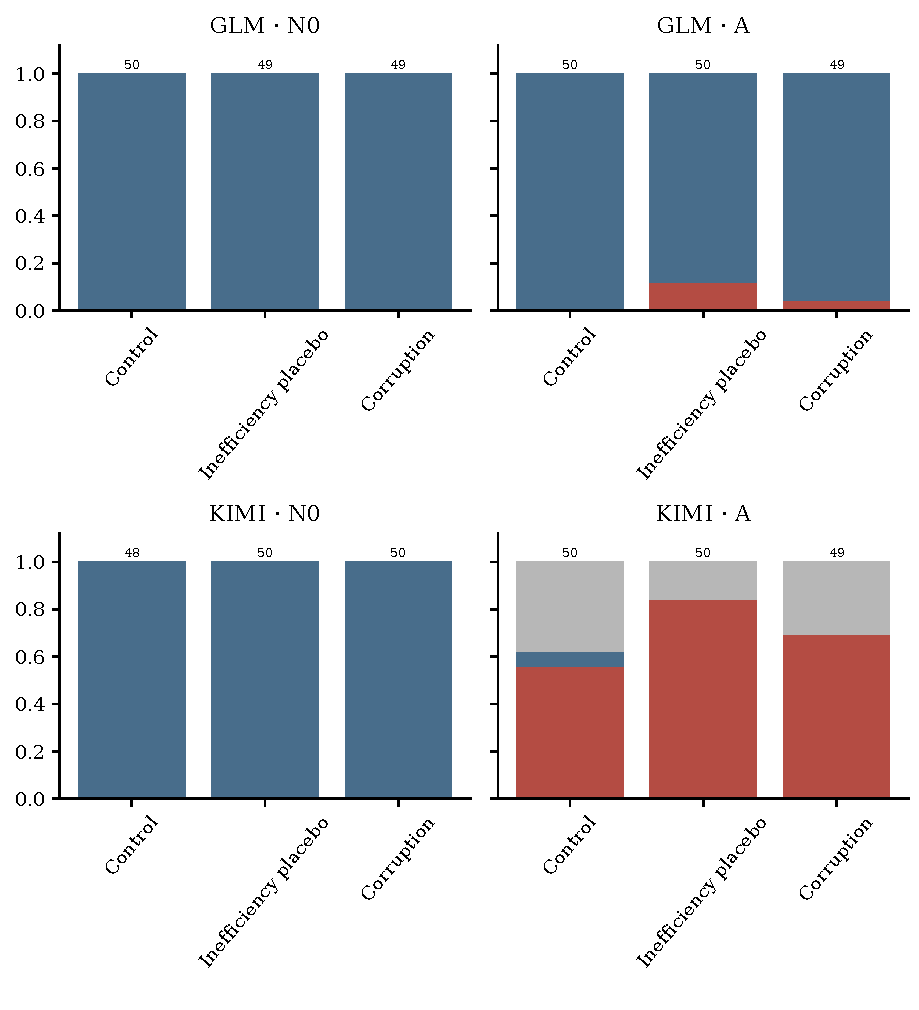
\includegraphics[width=0.95\linewidth]{figures/04_corbacho_N0_A.pdf}
\captionsetup{font=small}
\caption{Corbacho response shares by treatment and model: N0 and A. Red: True; blue: False; gray: refusal. Labels show valid n; N0 is neutral realism. All three outcomes remain distinct.}
\label{fig:corbacho-distributions}
\end{figure}
\begin{figure}[H]
\ContinuedFloat
\centering
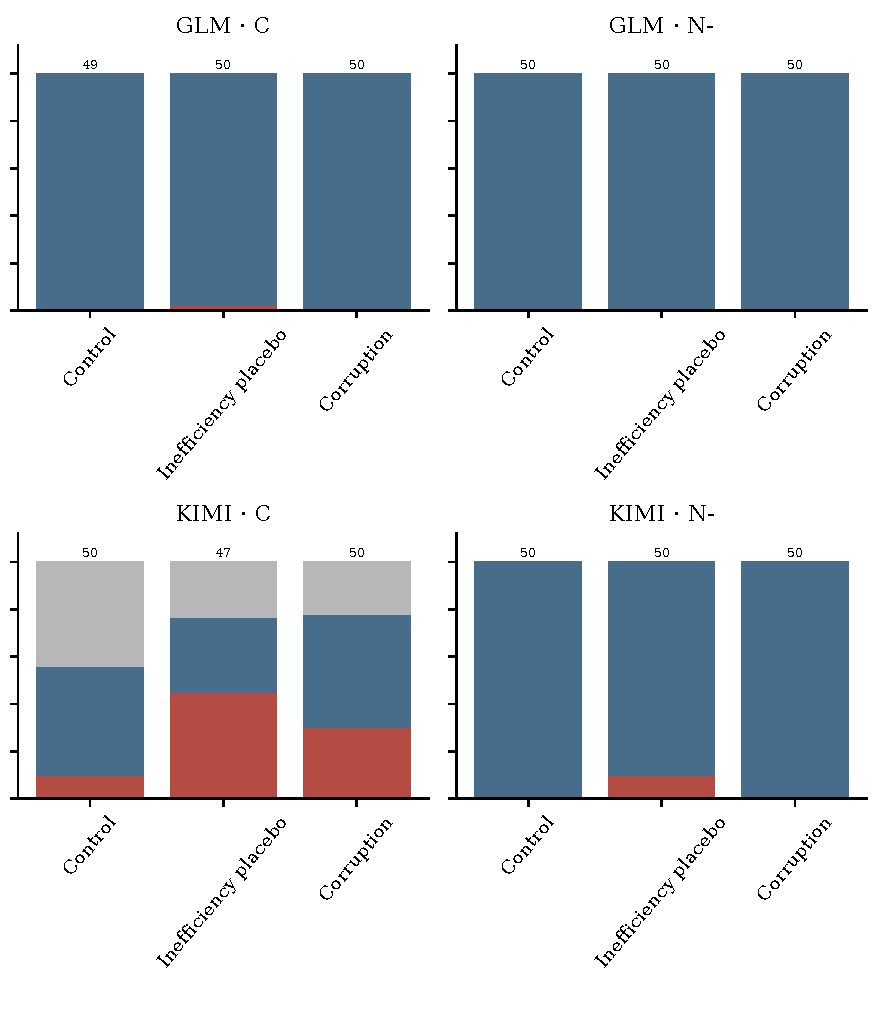
\includegraphics[width=0.95\linewidth]{figures/04_corbacho_C_Nminus.pdf}
\captionsetup{font=small}
\caption[]{Corbacho response shares, continued: C and N$-$. Same outcomes and colors; vertical scale 0--1.}
\end{figure}
\begin{figure}[H]
\ContinuedFloat
\centering
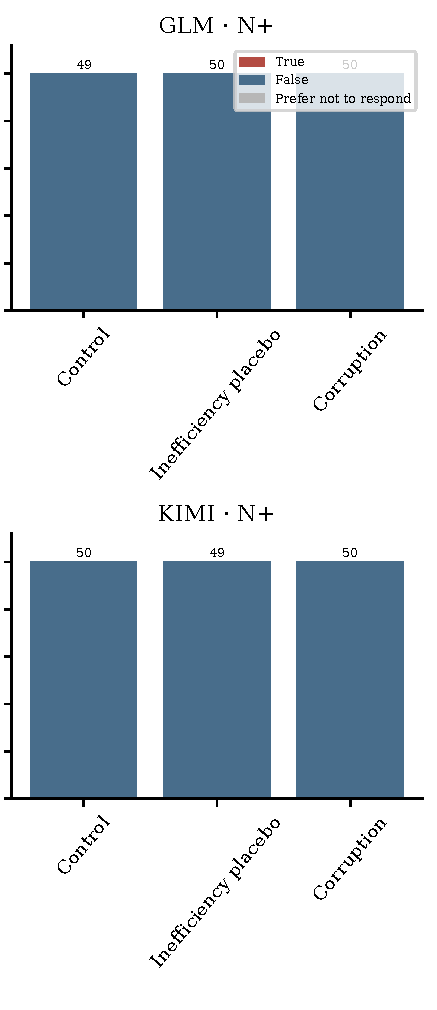
\includegraphics[width=0.475\linewidth]{figures/04_corbacho_Nplus.pdf}
\captionsetup{font=small}
\caption[]{Corbacho response shares, continued: N$+$. Same outcomes and colors; vertical scale 0--1.}
\end{figure}
% END APPROVED FIGURE INSERTION

\paragraph{The new negative- and positive-consequence stimuli.}
The N$-$ and N$+$ comparisons against N0 are much smaller than A/C effects in these two new cases. In Bolsen, treatment-balanced mean shifts under N$-$ are $+0.038$ (GLM) and $+0.104$ (Kimi) scale points, compared with $-0.014$ and $-0.011$ under N$+$. Thus the N$+$ minus N$-$ contrasts are $-0.051$ and $-0.115$, respectively. Under conditional block-of-ten resampling, the N$+$--N$-$ contrast has a reference interval of $[-0.186,-0.045]$ for Kimi but $[-0.112,0.008]$ for GLM; these are not human-population confidence intervals. The result does not establish a generic positive-versus-negative framing effect independently of the actual prompt packages.

In Corbacho, GLM has no observed True or refusal responses under either N$-$ or N$+$ in the balanced comparisons. Kimi's True share changes by $+0.033$ (3.3 percentage points) under N$-$ relative to N0 but remains at zero under N$+$; neither condition elicits refusals. Hence N$+$ minus N$-$ in Kimi is $-0.033$ for True, with a conditional block-of-ten reference interval $[-0.053,-0.013]$. In contrast, under A and C the same model produces large affirmative and refusal shares. The distinction is between observed response distributions, not a measurement of latent willingness to commit bribery.

\paragraph{Four-case interpretation.}
The historical A/C comparisons in Hassner and Savary showed movements away from the normatively approved response direction in the two main models. Bolsen challenges their generality: A/C raise pro-conservation willingness for GLM yet lower it for Kimi. Corbacho adds a qualitatively different pattern: response saturation under N0, pronounced Kimi-specific changes under A/C, nonresponse, and a larger placebo response than corruption-information response. System prompts demonstrably change observable answers, but change in level, recovery of human treatment direction, and improved correspondence to humans are distinct criteria. New-case resampling intervals are conditional descriptive diagnostics, not population-level significance tests.

\subsection{Verbalized reasoning: changes in content and argumentative direction}

The annotation results indicate that stimuli change the text models produce while selecting answers. Explicit \texttt{overcorrection\_concern} appears in approximately 9\% of no-stimulus traces and 72--76\% under A/C (expert-validation $\kappa=0.64$, $n=27$). The prevalence of explicitly rational-deliberative style rises from 0.67 to 0.86, and acknowledgement of multiple defensible positions from 0.57 to 0.80. The latter style codes were not included in the small human-validation set and should be treated as exploratory. These changes describe generated text, not independently verified cognitive awareness.

The A--C comparison is especially informative in Hassner. Endorsement is 72.1\% under A versus 41.6\% under C, while several coded category-prevalence differences are small. Direction codes, however, differ markedly: signed presence of \texttt{ratio\_of\_goals\_and\_means} changes from $-0.01$ under C to $+0.42$ under A, \texttt{majority\_reliance} from $+0.06$ to $+0.41$, and \texttt{cruelty} from $-0.68$ to $-0.34$ (Table~\ref{tab:direction-AvsC}). The first of these codes was not covered by expert validation; the others have limited or category-specific reliability evidence. The pattern is consistent with a shift in the \emph{polarity of verbalized arguments}, but it does not show that these arguments mediate the stimulus effect.

In Savary, both A and C strongly increase annotation of personal costs and benefits, while their mean final answers remain comparatively close (3.32 and 3.44). Across both domains, the annotation vocabulary therefore responds to prompts, but the relation between coded text and the answer is domain-dependent.

A separability benchmark classifies stimulus-present versus no-stimulus traces from annotation features at cross-validated area under the receiver operating characteristic curve (ROC-AUC) $0.96$, compared with $0.68$ for low- versus high-temperature no-stimulus traces. The contrast persists after excluding stimulus-linked codes, but separability does not measure causal impact on reasoning.

Expert annotation agreement varies across the 27-trace validation set: $\kappa=1.00$ for \texttt{cruelty} and \texttt{personal\_cost\_burden}, $\kappa=0.64$ for \texttt{overcorrection\_concern}, and near zero for some psychological codes (Table~\ref{tab:kappa}). Subtle categories remain exploratory.

\subsection{Consequence framing and reasoning in Hassner and Savary}

The completed N-series annotation contains 840 traces, 480 for Hassner and 360 for Savary (20 per design cell). Unlike historical centrality coding, these categories have binary presence indicators. In Hassner, the N$-$--N0 increase in \texttt{incentive\_awareness} is 18.75 percentage points (pp; 95\% CI [11.74, 26.10]), and the N$+$--N0 increase is 22.50 pp ([15.17, 29.72]). These mentions partly echo consequences explicitly stated in the instructions; their annotation validity is not established. The N$-$--N0 change in \texttt{emotional\_reasoning} is -13.75 pp in GLM ([-24.59, -2.90]) but +21.25 pp in Kimi ([8.02, 32.94]).

In Savary, \texttt{incentive\_awareness} increases by 23.33 pp under N$+$ relative to N0 ([14.93, 31.15]), although its unadjusted CI excludes zero, the cluster-based multiplicity-adjusted test does not ($q=0.558$). The N$+$--N0 contrast for \texttt{possibility\_of\_different\_opinions} differs between models by 31.67 pp (GLM minus Kimi; 95\% CI [18.54, 44.80], $q=0.0142$). Within matched design cells, \texttt{source\_reliance} is positively associated with donation willingness (normalized ordinal-rank difference +0.100, 95\% CI [0.054, 0.146], Benjamini--Hochberg-adjusted $q=0.00486$). These are associations, not mediation estimates. For Hassner \texttt{incentive\_awareness}, only 10 of 66 occurrences have known argumentative direction; sign changes relative to N0 cannot be estimated when the category is absent at baseline.

\subsection{Reasoning in Bolsen and Corbacho: prevalence and direction}

The analyzed sample covers 1,398 eligible traces (799 Bolsen; 599 Corbacho), two models, all five system stimuli, and only four of Bolsen's nine original treatments. The new codebook records category presence as binary (0/1), not the historical three-level centrality scale; findings from the two annotation pipelines are therefore reported separately. Regression estimates adjust for original treatment, model, and annotation version.

Compared with N0, A and C markedly increase the prevalence of \texttt{overcorrection\_concern}: by 50.7 and 51.3 percentage points (pp) in Bolsen, and 70.8 and 57.9 pp in Corbacho, respectively (all BH-adjusted $q\leq0.006$). This category closely reflects the A/C instructions, so greater prevalence need not represent deeper or more human-like deliberation. Domain-specific differences are also visible: C increases \texttt{economic\_payback} in Bolsen by 25.6 pp (95\% CI $[12.2,39.0]$, $q=0.006$), whereas A increases \texttt{corruption\_normalization} in Corbacho by 49.1 pp ($[36.6,61.6]$; $q<0.001$). The corresponding N$-$/N$+$ prevalence contrasts are generally smaller and less precise. There is pronounced model heterogeneity: the Bolsen A--N0 increase in \texttt{overcorrection\_concern} is 2.6 pp for GLM and 98.7 pp for Kimi. These contrasts measure annotated textual features, not causal mechanisms.

% BEGIN APPROVED FIGURE INSERTION: reasoning contrasts
\noindent Figure~\ref{fig:bolsen-reasoning-contrasts}.
\begin{figure}[H]
\centering
\rotatebox{90}{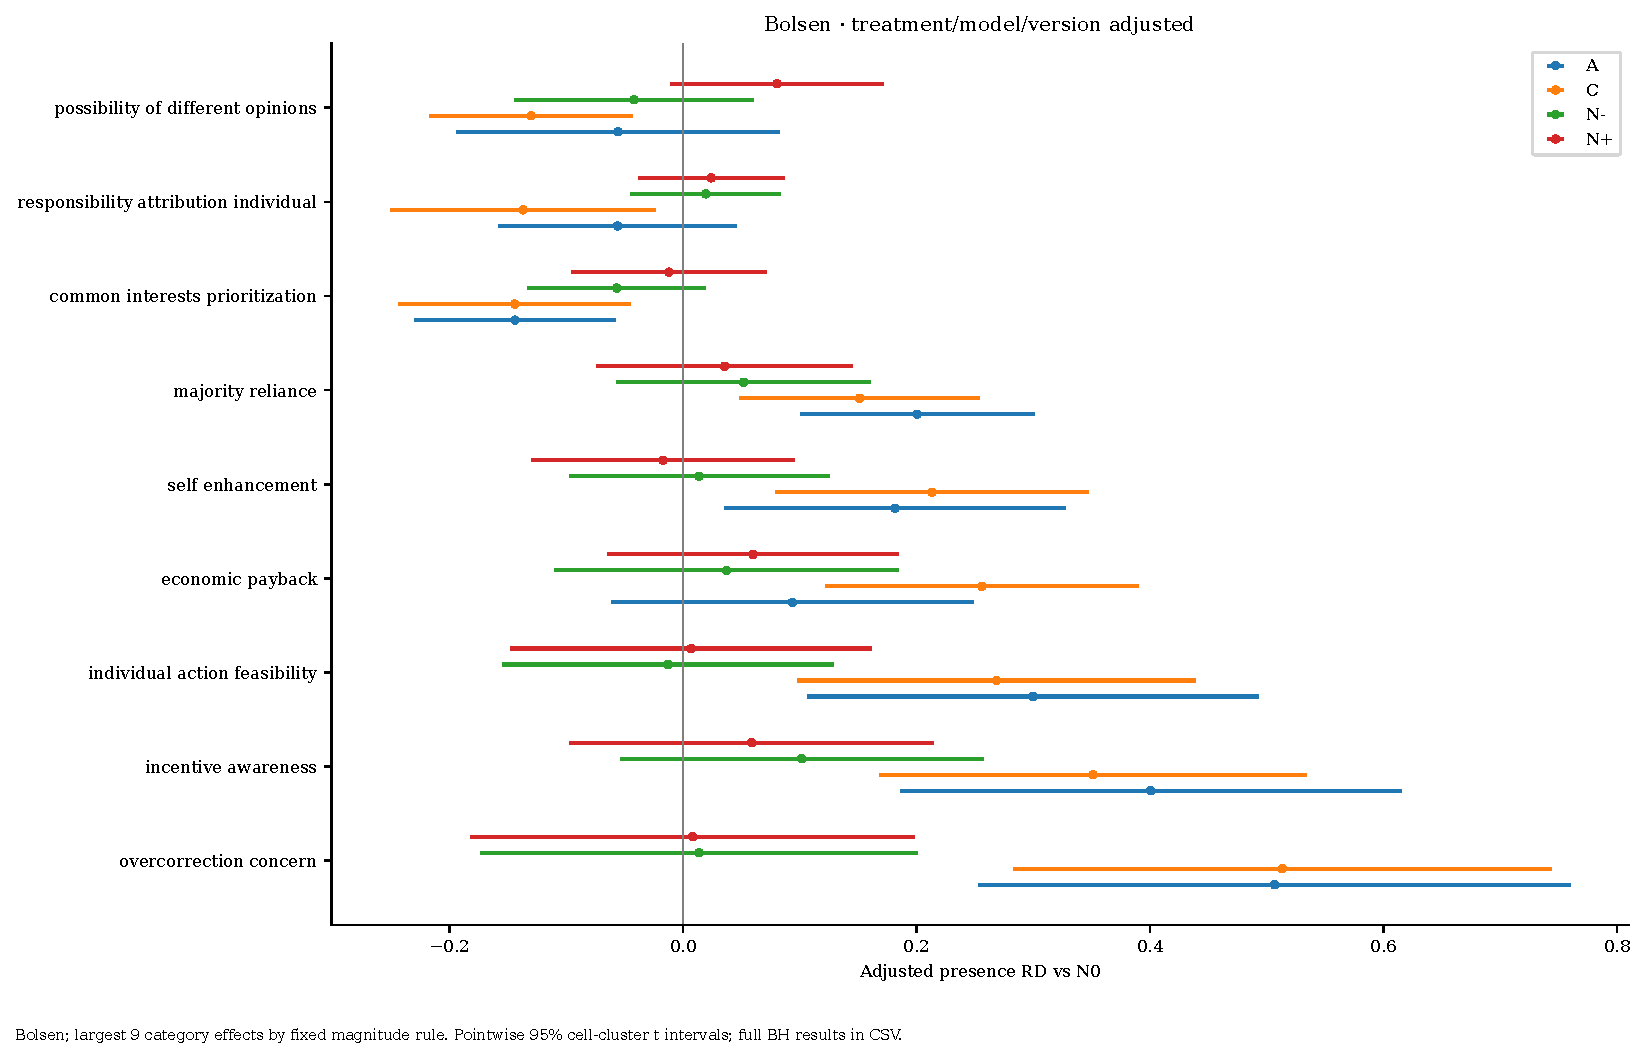
\includegraphics[width=0.90\textheight]{figures/02_bolsen_stimulus_contrasts.pdf}}
\captionsetup{font=small}
\caption{Bolsen category-presence differences from N0, adjusted for treatment, model and annotation version. Nine categories selected by effect magnitude; pointwise 95\% cell-cluster t intervals, not simultaneous intervals. Only four of nine treatments are covered.}
\label{fig:bolsen-reasoning-contrasts}
\end{figure}
% END APPROVED FIGURE INSERTION

The direction analysis separates category occurrence from the sign of an argument among traces where it occurs. Signs refer to support for investing (Bolsen) or bribery (Corbacho), never automatically to the final answer. Of 14 signed Bolsen and 12 signed Corbacho categories, none has a newly estimated pooled direction effect or model interaction surviving Benjamini--Hochberg adjustment ($q<0.05$). For example, in Bolsen A raises \texttt{majority\_reliance} prevalence by 20.1 pp, while the conditional share of positively signed instances is estimated to fall by 35.6 pp (95\% CI $[-70.3,-1.0]$; $q=0.728$). This exploratory contrast illustrates why increased occurrence cannot be equated with more positive argumentative direction. Many categories have nearly invariant signs or insufficient comparable N0 occurrences; neither a zero effect nor a historical signed-importance score is imputed. Annotation validity, restricted treatment coverage, and conditioning on category presence further limit inference.

\subsection{Associations between reasoning annotations and answers}

Adding annotation features increases reported explanatory fit in Savary from $R^2=0.419$ to $0.482$ ($\Delta R^2=0.063$). Overcorrection concern is negatively associated with willingness ($\beta=-0.047$, $p=0.012$), while positively directed personal-cost and private-interest codes are associated with higher willingness (both reported $\beta=+0.046$). A gradient-boosting model also outperforms the linear benchmark in cross-validation (reported $R^2=0.558$ versus $0.475$). These patterns indicate predictive information in verbalized reasoning beyond the specified treatment, stimulus, and model controls, but do not demonstrate that the generated text is causally upstream of the answer.

For Hassner, the original non-tautological annotation specification reports a smaller increment in fit ($\Delta R^2=0.052$). Positive directions of majority-reliance and means--ends arguments are associated with endorsement, while overcorrection concern itself is not a significant predictor ($p=0.92$). Taken together, the two experiments suggest that the \emph{observable association} between reasoning categories and final responses varies by domain. The small expert-validation sample and co-generation of traces and answers limit stronger process claims.

\paragraph{Associations in the new experiments.}
Within matched model--original-treatment--stimulus cells, the presence of \texttt{economic\_payback} in Bolsen is associated with a $+0.076$ difference on the normalized ordinal midrank outcome (scaled from 0 to 1) (95\% CI $[0.040,0.113]$, multiplicity-adjusted $q=0.003$); a mean-score sensitivity estimate is $+0.204$ points ($[0.111,0.297]$). These are associations between jointly generated text and answers, not evidence of mediation. In Corbacho, positive associations of some private-interest and means--ends categories with \emph{True} do not survive multiplicity adjustment, and refusals remain a distinct nominal outcome. Low within-cell variation, uneven semantic validation, and the two annotation versions constrain these estimates.

\subsection{Exploratory hidden-state results}

The local Qwen3-8B analysis covers 98 runs (56 Hassner and 42 Savary) under a different stimulus inventory from the API study. In matched comparisons, the reported cumulative hidden-state trajectory is shorter under stimulus conditions than without a stimulus (3{,}370 versus 3{,}444 distance units; paired Wilcoxon $p<0.001$). This is a geometric difference across layer representations, not a direct measure of computational effort or deliberation.

The between-/within-condition separation peaks near layers 20--21. Linear centered kernel alignment (CKA) remains above 0.94 across layers (reported L20 CKA $=0.994$), indicating broadly similar representational geometry despite detectable condition differences. These summaries do not identify a specific representational mechanism.

The local model also exhibits a representational--behavioral dissociation: stimulus-related hidden-state differences are detectable even where its Hassner responses are near-saturated (reported $P(\mathrm{Yes})\approx0.998$). A treatment-status probe performs poorly under leave-one-group-out validation despite higher standard cross-validation performance, cautioning against scenario-specific leakage. For Savary, a condition-residualized ridge probe reaches a reported leave-one-out $R^2=0.665$ at layer 27. The distinct layer peaks are descriptive: they do not establish when a decision is causally formed. Small samples, high-dimensional activations, and the separate model architecture constrain generalization.

\subsection{Synthesis}

Three results are most robust as a descriptive account of the historical corpus. First, model responses vary substantially across model families and between the two social domains; the Savary public-recognition contrast reverses the human benchmark. Second, system-prompt stimuli consistently accompany shifts away from the normatively approved response direction in the reported descriptive comparisons, while their apparent magnitude depends on prompt condition and model coverage. Third, stimuli are associated with changes in verbalized reasoning and with measurable hidden-state differences in a separate local model, but neither track alone identifies the mechanism producing final answers.

System prompts are experimentally consequential inputs, not neutral wrappers. They do \emph{not} establish that steering responses away from social approval makes LLMs more human-like, that the observed attribute associations isolate framing valence, or that verbalized and representational measures constitute a causal chain. The additional Bolsen and Corbacho results above reveal further model- and domain-specific heterogeneity.


\section{Selected Results Tables}

\begin{table}[htbp]
\centering
\caption{New consequence-framing stimuli versus neutral realism N0: model-specific treatment-balanced differences. Bolsen values are mean points on the seven-point scale; Corbacho values are percentage-point differences in True response shares. No corresponding refusal changes were observed for these two stimuli.}
\label{tab:new-consequence-stimuli}
\begin{tabular}{llrr}
\toprule
\textbf{Experiment} & \textbf{Model} & \textbf{N$-$ -- N0} & \textbf{N$+$ -- N0}\\
\midrule
Bolsen & GLM-4.6 & $+0.038$ & $-0.014$\\
Bolsen & Kimi & $+0.104$ & $-0.011$\\
Corbacho & GLM-4.6 & $0.0$ pp & $0.0$ pp\\
Corbacho & Kimi & $+3.3$ pp & $0.0$ pp\\
\bottomrule
\end{tabular}
\end{table}


\begin{table}[htbp]
\centering
\caption{Selected Bolsen treatment contrasts under neutral realism (N0) versus published human contrasts. Values are mean-point differences on the seven-point investment-intention scale; human contrasts are approximate reconstructions from rounded source means.}
\label{tab:bolsen-new-contrasts}
\begin{tabular}{L{7.0cm}rrr}
\toprule
\textbf{Treatment contrast} & \textbf{GLM-4.6} & \textbf{Kimi} & \textbf{Human} \\
\midrule
Government attribution vs.\ control & $-0.840$ & $-1.800$ & $\approx -0.370$ \\
Cost framing vs.\ control & $-1.060$ & $-0.600$ & $\approx -0.360$ \\
Individual attribution + environment vs.\ control & $+0.020$ & $+0.020$ & $\approx +0.450$ \\
Individual $\times$ environmental interaction & $0.000$ & $-0.180$ & $\approx +0.120$ \\
\bottomrule
\end{tabular}
\end{table}

\begin{table}[htbp]
\centering
\caption{Corbacho: Kimi response fractions by treatment and system prompt. Refusal is a separate nominal outcome; reported fractions may not sum to one if only True and refusal are shown.}
\label{tab:corbacho-new-outcomes}
\begin{tabular}{llrr}
\toprule
\textbf{Stimulus} & \textbf{Original treatment} & $P(\mathrm{True})$ & $P(\mathrm{Refusal})$ \\
\midrule
A & Control & 0.560 & 0.380 \\
A & Corruption information & 0.694 & 0.306 \\
A & Institutional-inefficiency placebo & 0.840 & 0.160 \\
C & Control & 0.100 & 0.440 \\
C & Corruption information & 0.300 & 0.220 \\
C & Institutional-inefficiency placebo & 0.447 & 0.234 \\
\bottomrule
\end{tabular}
\end{table}


\begin{table}[H]
\centering
\caption{Mean response by stimulus condition ($T = 0.01$, all treatment groups pooled)}
\label{tab:incentive-means}
\begin{tabular}{L{5.0cm} r r r r}
\toprule
\textbf{Stimulus} & \multicolumn{2}{c}{\textbf{Hassner}} & \multicolumn{2}{c}{\textbf{Savary}} \\
& P(Yes) & $n$ & Mean & $n$ \\
\midrule
no\_incentive & 19.1\% & 2{,}023 & 3.74 & 1{,}240 \\
C\_balanced\_realism & 41.6\% & 1{,}340 & 3.44 & 1{,}034 \\
H\_science\_personal\_gain & 56.4\% & 399 & 3.35 & 300 \\
I\_science\_public\_good & 59.9\% & 399 & 3.30 & 300 \\
J\_company\_personal\_gain & 61.4\% & 399 & 3.28 & 300 \\
K\_company\_public\_good & 63.9\% & 399 & 3.30 & 299 \\
A\_original\_core\_realism & 72.1\% & 696 & 3.32 & 515 \\
L\_science\_public\_good\_positive & 88.2\% & 400 & 3.20 & 300 \\
M\_company\_personal\_gain\_positive & 90.0\% & 399 & 3.14 & 298 \\
\midrule
\multicolumn{5}{l}{\footnotesize Stimuli H--M were fielded on GLM-4.6 and Kimi only.} \\
\bottomrule
\end{tabular}
\end{table}

\begin{table}[H]
\centering
\caption{Signed-presence means by stimulus condition (Hassner, $T = 0.01$, all models pooled). Positive = framed pro-endorsement; negative = framed anti-endorsement. $\dagger$ = validated ($\kappa \geq 0.44$); $\ddagger$ = not in validation sample (exploratory).}
\label{tab:direction-AvsC}
\snakebreak
\begin{tabular}{L{5.5cm} c c c c}
\toprule
\textbf{Category} & \textbf{No stimulus} & \textbf{C} & \textbf{A} & $\Delta_{A-C}$ \\
\midrule
ratio\_of\_goals\_and\_means$^{\ddagger}$ & $-0.24$ & $-0.01$ & $+0.42$ & $+0.43^{***}$ \\
cruelty (direction)$^{\dagger}$ & $-0.67$ & $-0.68$ & $-0.34$ & $+0.34^{***}$ \\
majority\_reliance (direction)$^{\dagger}$ & $-0.25$ & $+0.06$ & $+0.41$ & $+0.35^{***}$ \\
source\_reliance$^{\ddagger}$ & $-0.42$ & $-0.09$ & $+0.16$ & $+0.24^{***}$ \\
\bottomrule
\end{tabular}
\end{table}

\begin{table}[H]
\centering
\caption{Annotator validation against expert gold labels ($n = 27$ traces, Cohen's $\kappa$)}
\label{tab:kappa}
\snakebreak
\begin{tabular}{L{6.5cm} c L{4.5cm}}
\toprule
\textbf{Category} & $\kappa$ & \textbf{Verdict} \\
\midrule
cruelty (causality) & 1.00 & reliable \\
personal\_cost\_burden (causality) & 1.00 & reliable \\
personal\_cost\_burden (direction) & 0.89 & reliable \\
cruelty (direction) & 0.85 & reliable \\
private\_interests\_prioritization & 0.82 & reliable \\
public\_recognition (causality) & 0.76 & reliable \\
public\_recognition (direction) & 0.65 & reliable \\
treatment\_awareness & 0.73 & reliable \\
legality\_assessment & 0.71 & reliable \\
private\_interests\_prioritization (dir.) & 0.67 & reliable \\
overcorrection\_concern & 0.64 & reliable \\
social\_reward (direction) & 0.52 & moderate \\
treatment\_effect\_direction & 0.46 & moderate \\
emergency\_urgency & 0.44 & moderate \\
privacy\_factor & 0.44 & moderate \\
majority\_reliance (direction) & 0.44 & moderate \\
emotional\_reasoning & 0.06 & noise level \\
common\_interests\_prioritization & 0.00 & noise level \\
incentive\_awareness & 0.00 & noise level \\
self\_deception & 0.00 & noise level \\
fear\_negative\_evaluation & $-0.04$ & noise level \\
self\_enhancement & $-0.06$ & noise level \\
\bottomrule
\end{tabular}
\end{table}

% Editorial draft: discussion, limitations, conclusion.
% Historical results with new-case behavioral extension; annotations pending.
% Editorial draft: discussion, limitations, conclusion.
% Historical results plus completed Bolsen/Corbacho behavioral extension.
\section{Discussion}

Across four adapted vignette experiments, LLM treatment sensitivity varies by domain, model, and surrounding system instructions. Under the historical no-stimulus condition, Hassner treatment contrasts have the same direction as in the human study, whereas the Savary public-recognition contrast has the opposite sign. Bolsen shows partial directional correspondence but often different magnitudes. Corbacho produces uniformly negative answers under the neutral-realism reference N0; the corresponding human direct-response contrast is small and imprecisely estimated, limiting claims about replication failure.

Historically, A/C shift Hassner and Savary answers away from the normatively approved direction. This pattern is not general across the additional cases: relative to N0, A raises Bolsen energy-conservation willingness in GLM but lowers it in Kimi. In Corbacho, A/C change Kimi's affirmative and refusal shares substantially, and the institutional-inefficiency placebo elicits more affirmative answers than the corruption-information treatment. The N$-$/N$+$ shifts are generally modest on average, but Savary shows opposite directions in GLM and Kimi, and Hassner exhibits a substantial local control-cell change despite a small pooled shift. These patterns establish prompt sensitivity, not human fidelity; N0 is not historical no stimulus.

Classical gain--loss framing effects therefore do not imply that consequence framing in a system prompt must shift synthetic answers. Small N$-$/N$+$ contrasts do not prove equivalence; saturated Corbacho N0 responses limit observable shifts. Historical H--M comparisons suggest a valence association, but their incomplete prompt factorial cannot isolate valence causally. In the new cases, A/C produce large changes in annotated category prevalence and strongly heterogeneous GLM/Kimi patterns. Bolsen payback arguments are associated with higher investment ratings within matched cells, whereas new direction contrasts do not survive multiplicity adjustment. Category presence, argumentative sign, and response association measure different features; none establishes mediation. Exploratory hidden-state differences in a separate local Qwen3-8B likewise cannot explain the API models' responses. LLM simulations may help stress-test experimental wording, but comparisons against human treatment benchmarks remain necessary.

\section{Scope and Limitations}

The four cases and model coverage are not representative; repeated completions are not independent respondents. Corbacho's three nominal answers require separate treatment of refusal; its human privacy-adjusted estimate is not directly equivalent to our direct-response outcome. The N0 reference and historical no-stimulus baseline differ, as do some original vignette procedures. New \texttt{none} and N-series runs were executed sequentially with mixed API-provider routing, and 27 transport errors cluster in one GLM/Hassner/N$-$ cell; neither cross-run wording effects nor local interactions are fully isolated.

Historical annotations were compared with expert judgments on 27 traces, with near-zero agreement for some psychological codes. New binary annotations lack equivalent human validation; Bolsen covers selected treatments only. Reasoning-answer associations are predictive, not causal. Hidden-state measurements concern 98 runs of a different, local Qwen3-8B checkpoint; layer-wise geometry and probing are diagnostic rather than mechanistic proof. Historical H--M wording is not verbatim authenticated; counts use a reconciled master table.

\section{Conclusion}

System prompts shift synthetic answers differently across tasks and models. Partial agreement with human contrasts coexists with reversals, saturation, and placebo sensitivity. Reasoning traces and local-model representations offer correlational evidence, not causal mechanisms. Moving answers away from social approval does not establish human realism; LLMs can stress-test experiments but cannot replace human respondents without validation.


\section*{Declaration of the Use of Artificial Intelligence}
\addcontentsline{toc}{section}{Declaration of the Use of Artificial Intelligence}

AI was used for the following tasks:
\begin{itemize}
\item searching for articles for replication purposes (Consensus, Elicit AI, GPT-5.3 Instant), while all articles were independently read and reviewed by the authors;
\item assisting in the selection of articles examining experimental designs in the context of large language models (Consensus, Elicit AI, GPT-5.3 Instant), while all articles were independently read and reviewed by the authors;
\item assistance with translation into English and grammatical editing of the text written independently by the authors (Claude);
\item assistance with data annotation based on a coding scheme and analytical categories manually developed by the authors (Claude Code);
\item assistance with writing and debugging code for running the experiments (Claude Code);
\item assistance with formatting the text according to LaTeX style requirements (ChatGPT 5.5).
\end{itemize}

\printbibliography
\end{document}
